%%%%%%%%%%%%%%%%%%%%%%%%%%%%%%%%%%%%%%%%%%%%%%%%%%%%%%%%%%%%%%%%%%%%%%%%%%
%%%%%                         CHAPITRE 7                            %%%%%%
%%%%%%%%%%%%%%%%%%%%%%%%%%%%%%%%%%%%%%%%%%%%%%%%%%%%%%%%%%%%%%%%%%%%%%%%%%

\lhead[\fancyplain{}{\leftmark}]%Pour les pages paires \bfseries
      {\fancyplain{}{}} %Pour les pages impaires
\chead[\fancyplain{}{}]%
      {\fancyplain{}{}}
\rhead[\fancyplain{}{}]%Pour les pages paires 
      {\fancyplain{}{\rightmark}}%Pour les pages impaires \bfseries
\lfoot[\fancyplain{}{}]%
      {\fancyplain{}{}}
\cfoot[\fancyplain{}{\thepage}]%\bfseries
      {\fancyplain{}{\thepage}} %\bfseries
\rfoot[\fancyplain{}{}]%
     {\fancyplain{}{\scriptsize}}


%%%%%%%%%%%%%%%%%%%%%%%%%%%%%%%%%%%%%%%%%%%%%%%%%%%%%%%%%%%%%%%%%%%%%%%%%%
%%%%%                      Start part here                          %%%%%%
%%%%%%%%%%%%%%%%%%%%%%%%%%%%%%%%%%%%%%%%%%%%%%%%%%%%%%%%%%%%%%%%%%%%%%%%%%

\chapter{Capturing equipment along with the athlete - Application to BMX racing}
\label{ch:7}

%==============================================================================	Résumé du chapitre

\begin{center}
\rule{0.7\linewidth}{.5pt}
\begin{minipage}{0.7\linewidth}
\smallskip

\textit{Numerous sports disciplines are practiced with special equipment, such as a board in skateboarding, a racket and a ball in tennis, or a bike in BMX racing. The interactions between the athlete and their gear are often important to retrieve. We analyzed a BMX start sequence, by using OpenPose for 2D human pose estimation, and a custom trained DeepLabCut model for bike detection. We ran Pose2Sim on the joint {pilot+bike} 2D estimations, and performed 3D inverse kinematics on a custom OpenSim {pilot+bike} model. This showed that analyzing simultaneously the athlete and their equipment is possible, which provides additional perspectives for markerless sports motion analysis.\newline
See Figure~\ref{fig_visabstract5} for a visual abstract.
}

%\smallskip
\end{minipage}
\smallskip
\rule{0.7\linewidth}{.5pt}
\end{center}

\newpage

\minitoc

\vspace*{3cm}

\begin{figure}[hbtp]
	\centering
	\def\svgwidth{1\columnwidth}
	\fontsize{10pt}{10pt}\selectfont
	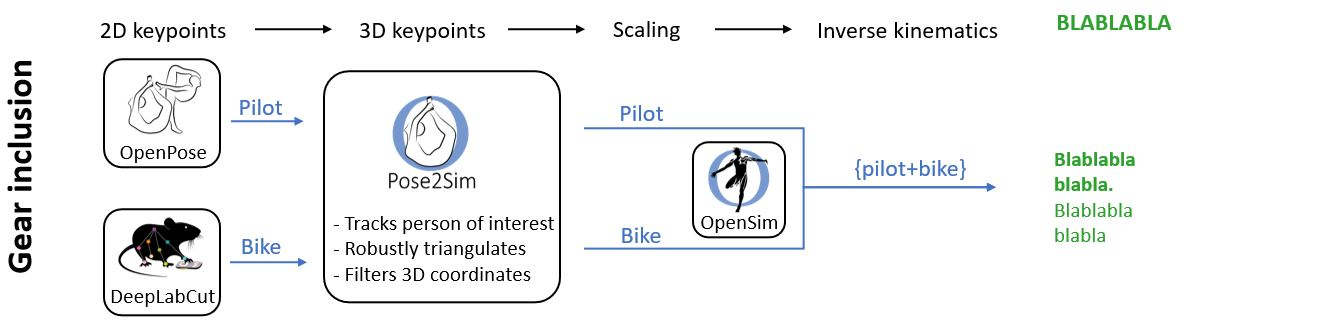
\includegraphics[width=\linewidth]{"../Intro/Figures/Fig_VisAbstract5.JPG"}
      \caption{Visual abstract for joint analysis of the athlete with OpenPose, and their equipment with DeepLabCut.}
	\label{fig_visabstract5}
\end{figure}

\newpage


\section{Introduction}
\subsection{The importance of equipment}

Numerous sports disciplines involve equipment; and sometimes, the motion of this equipment and of the athlete are of equal importance. Tracking a ball in soccer can help understand anticipated actions and game dynamics \cite{Ghasemzadeh2021}, documenting the motion of a tennis racket \cite{Martin2013}, a hockey stick \cite{Kays2017} or oars of a rowing boat \cite{Ruffaldi2015} gives insight on the interactions between the athlete and their gear, and retrieving information about skis \cite{Ludwig2020} or bike parts \cite{Rosenhahn2008} can help quantify specific posture cues.

However, this is challenging on several levels. First, the equipment needs to be tracked. This is straightforward with marker-based or IMU based technologies: one can simply equip the object with an additional marker, or sensor. However, this is more complicated with a markerless approach based on deep-learning, as it involves labelling each point or object of interest on numerous images, and training a specific model. Second, in case the equipment is multisegmented, its own kinematics needs to be calculated, either with a 6DoF approach, or via inverse kinematics. In the latter case, a specific model needs to be crafted, with accurate joint specifications and segment dimensions. Third, when the athlete is in contact with their equipment, it can be interesting to solve the combined kinematics of the whole $\{athlete+equipment\}$ system. The problem remains simple if the kinematic chain remains open like in a tennis serve \cite{Martin2013}, however when the equipment makes it a closed loop, this can become rapidly much more complex, and the privileged solution consists in modeling the kinematic chain as a set of open chains, constrained together \cite{Rosenhahn2008}. 

BMX race represents such a problem. Coaches are interested in the motion of the bike as regards to the athlete. As a consequence, the bike needs to be tracked, modeled, and then its kinematics needs to be computed. This is especially difficult, because both feet and both hands are in contact with the bike, which makes it a particularly constrained closed chain, hence very difficult to solve. 


\subsection{The start in BMX racing}
BMX race differs from other cycling disciplines in different ways, one of them being the short duration and of each race. At the elite level, they last about 30 to 40 seconds \cite{Cowell2012}. Hence, the winner is the one who has not only averaged the greatest speed, but also taken the shortest trajectory. In order to be able to choose the best one without being obstructed by other riders, one has to take a good start. \cite{Rylands2014} analyzed the statistics of 348 elite racers in UCI (Union cyclist international) competitions, and found a strong correlation between early placing and final placing. Most authors actually study the start, rather than any other part of the race \cite{Zabala2009,Gianikellis2011,Chiementin2012,Kalichova2013,Rylands2014}.

Moreover, riders never sit on their saddle. When cycling off the saddle in road cycling, arms have been shown to be more involved since they push and pull the handlebar \cite{Stone1993}, as the body is brought upward and forward over the axis of crank rotation. Hence, this discipline requires conducting whole body analysis. \cite{Gianikellis2011} suggest that for a faster start, the Range Of Motion (ROM) of the knee needs to be smaller than that of the trunk. \cite{Kalichova2013} finds a clear asymmetry in upper-body motion, both in terms of elbow and shoulder joint angles. However, as these two are case studies, it is hard to give much trust to these measurements in terms of performance. More specifically, the first movement initiated during a BMX start is the so-called "slingshot" maneuver. It consists in moving the body down and forward, while the bike goes in the opposite direction, the front wheel lifting noticeably. This plyometric countermovement occurs before the first pedal stroke, and before the gate has entirely dropped. According to \cite{Gross2017}, this technique is highly effective. It involves a stretch-shortening cycle of the front knee, and the counter-movement is more pronounced and initiated earlier in better riders. This confirms that the complex motion of the bike as regards to the pilot at start is of crucial importance (see Figure~\ref{fig_bmxstart}). 

\cite{Grigg2017} concludes her literature review by underlying that research associating kinematic characteristics and gate start performance would be useful for coaches. She also adds that both equipment and rider analysis are of critical importance. Finally, she points out that research should be done on-field, rather than in lab conditions which would introduce bias. As a consequence, we captured the start in BMX race, in ecologically valid conditions, tracking both the pilot and the bike movement in 3 dimensions, with a markerless protocol. The goal was to propose a method for such an objective, and verify whether some kinematic variables could be measured.

\begin{figure}[hbtp]
	\centering
	\def\svgwidth{1\columnwidth}
	\fontsize{10pt}{10pt}\selectfont
	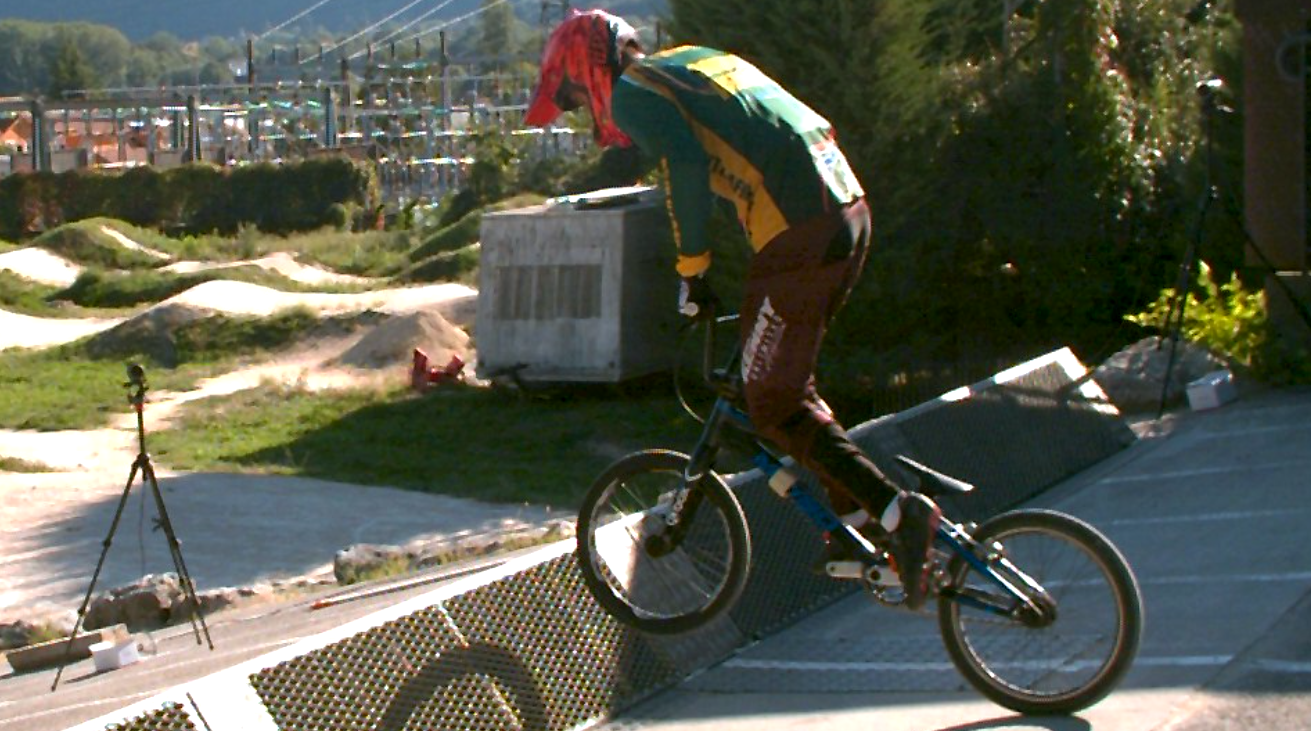
\includegraphics[width=\linewidth]{"../Chap7/Figures/BMXStart.PNG"}
	\caption{The early slingshot maneuver in BMX race.}
	\label{fig_bmxstart}
\end{figure}


\section{Methods}

\subsection{Material and protocol}
As this was a preliminary experiment, we conducted this study on one single pilot, and examined one single start. Only 6 Qualisys Miqus cameras were used. The resolution was only of 1 megapixel, however the framerate was of 120 fps. Synchronization was achieved with a hardware trigger, but calibration was not successful with the standard method using a wand equipped with markers. In broad daylight, markers were either missing, or confused with artifact reflections. Hence, we calibrated on the grid dimensions, in the same way as described in previous chapter (see \nameref{calib_pnp}). Calibration was not as accurate as it would have been with a gold-standard method, but it remains in the centimetric order of magnitude.

The amateur pilot involved in this study signed a form of informed consent. He was first captured standing on a T-pose for scaling the skeletal OpenSim model accordingly, and then performed 3 starts in conditions similar to those of a competition. He was accustomed to the BMX track and the 5 meters starting hill, as well as with the standard gate and sound signal used for setting off the start. He wore his usual equipment, and confirmed that his movement and concentration were not hindered by the capture. Among the 3 starts the pilot executed, only one of them was studied. 


\subsection{Pilot inverse kinematics}


J'EN SUIS LA




\subsection{Bike inverse kinematics}

Voir thèse Princelle

% This can be done, for example, by separately process the video with OpenPose, as well as with a custom-trained DeepLabCut model. 
% Resulting .trc coordinate files can be merged, and used in OpenSim. However, the DeeLabCut keypoints must be referenced on an OpenSim model, which may need to be crafted from scratch, such as a ball, skis, or bike, depending on the detected object.
% Détection OpenPose : c'est vraiment pas terrible : on n'a que 6 caméras, de qualité pas terrible, et l'équipement et les occlusions lui rendent vraiment la vie difficile.
% DeepLabCut c'est pareil (j'ajouterais que je pourrais sûrement affiner l'entraînement pour avoir des résultats légèrement meilleurs).
% Dans tous les cas, même en triturant tous les paramètres possibles pour la triangulation Pose2Sim, j'ai des résultats très moyens.

% - Scaling : J'ai scalé le vélo et le pilote indépendamment, puis j'ai assemblé les deux.


\begin{figure}[hbtp]
	\centering
	\def\svgwidth{1\columnwidth}
	\fontsize{10pt}{10pt}\selectfont
	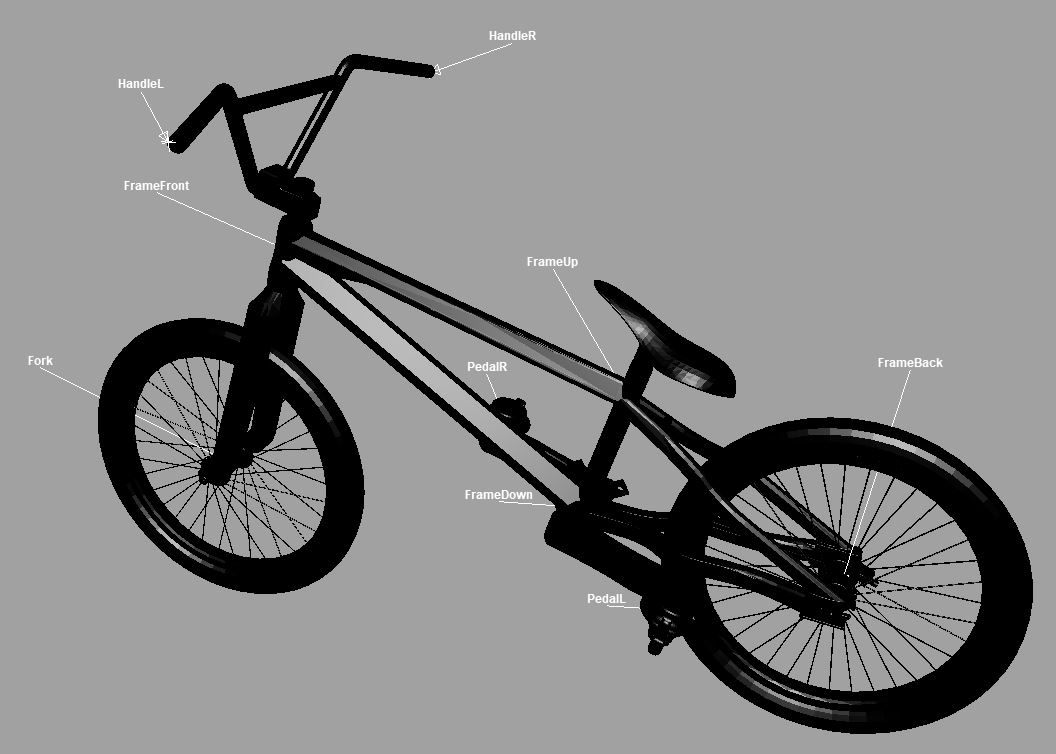
\includegraphics[width=\linewidth]{"../Chap7/Figures/Bike_keypoints.PNG"}
	\caption{The articulated bike model, and the labels DeepLabCut was trained to recognize.}
	\label{fig_bikemodel}
\end{figure}





\subsection{Joined pilot and bike inverse kinematics}
% Marche pas avec nos qualités de vidéo : simulations

% - Cinématique inverse : Ça marche si je relâche les contraintes entre le vélo et le pilote (mais dans ce cas, ça perd de son intérêt). 
% Ça marche aussi si j'utilise toutes les données marqueurs.
% Si je ne sélectionne que les marqueurs des centres articulaires et 9 marqueurs vélo (l'équivalent du workflow markerless s'il était assez exact), ça marche également.

% Par contre, en markerless et avec les contraintes entre le vélo et le pilote, ça ne fonctionne plus... J'ai essayé en changeant les poids, en relâchant les contraintes, en libérant les limites articulaires, rien à faire. 
% Le mieux que j'aie pu faire (cf gif), c'est avoir des résultats en n'utilisant que les contraintes pied/pédale (et pas celles mains/guidon). 
% image.png



\subsection{Performance indicators assessment}
Critères perf
- Pilot: Flexion of the front knee (Plyometric action), flexion of both elbows (asymmetric?)
- Bike: Elevation of the front wheel, handlebar angle
- Both: Forward Speed of the COM bike and pilot (diff directions, separate), Right foot and right pedal rotational excursion (constrained?) % (xped-xframe, yped-yframe), (xfoot-xframe, yfoot-yframe)




\begin{figure}[hbtp]
	\centering
	\def\svgwidth{1\columnwidth}
	\fontsize{10pt}{10pt}\selectfont
	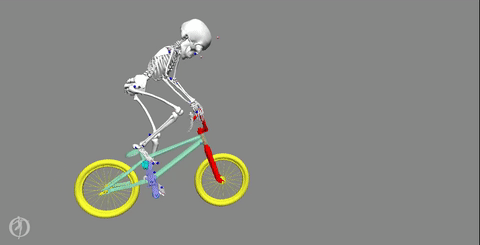
\includegraphics[width=\linewidth]{"../Chap7/Figures/BMXPilot.png"}
	\caption{Note that the head is only big because the pilot was scaled with his helmet on. Since the head is at the end of the kinematic chain, and as kinetics are not addressed, it does not affect inverse kinematics. See animated version \href{https://github.com/perfanalytics/pose2sim/blob/main/Content/Activities_verylow.gif}{here}.}
	\label{fig_bmxpilot}
\end{figure}

% \begin{frame}{Embedded Animation}
%   \animategraphics[loop,controls,width=0.7\linewidth]{25}{"../Chap7/Figures/bmxgif/bmx"}{1}{180}
% \end{frame}



\section{Results}



\section{Discussion}
\subsection{On these data}


\subsection{Limits and perspectives}

pre manip, 1 pilot 1 start, slt 6 cam, low res, calib unsuccessful

Rosenhahn2008 snowboard: closed kinematic chain: pas évident, voir [17] ( reduced equations of robotic systems using Lie groups). Eux: soft constraints (invariances -> numeric) rather than joints (analytic)

Formalisme joint vs constraint Part 3.1 https://sci-hub.se/https://ieeexplore.ieee.org/document/4587520

other leads: bushing forces, ball joints
scale avant et arriève vélo indépendament
% Because OpenSim models have fewer degrees of freedom than the human body, it is easy to define a set of constraints that seems very reasonable but is not easy for the skeleton (rigid-body mechanism) to satisfy.
% If it's appropriate for the movement you are simulating, you might consider allowing the toes and/or hands to rotate relative to the pedals
% (see PointConstraint, https://simtk.org/api_docs/opensim/api_docs/classOpenSim_1_1PointConstraint.html#details).
% Alternatively, you could attach the toes and/or hands to the bike via BushingForces (or sprint forces ?) (https://simtk.org/api_docs/opensim/api_docs/classOpenSim_1_1BushingForce.html#details).


% riders use a very particular technique for gaining speed in the bumps without pedaling, known as “pumping” 
% [Cowell 2012, Rylands 2016]: on the way up they decrease their loss in gravitational potential energy by bending their arms and legs, and on the way down they increase their kinetic energy by extending their limbs. Finally, athletes have to take big jumps and to operate sharp turns without colliding with each other. Unfortunately, according to [Novak & Dascombe 2014] the majority of performance characteristics studies have been conducted on road cycling athletes.  [Cowell 2012] shows that hip and knee extensors, as well as horizontal shoulder abductors and adductors are heavily relied upon all along the race. 



Mathis2020 Principles, pitfalls and perspectives

% ajouter video de use on your own data
splashes, occlusions, distance, etc

Voir Protocole doc: % https://1drv.ms/w/s!AvGG4T_aAnWzmy4JuQph05pIphXX?e=0yjqbs
